
\documentclass[10pt,fleqn]{beamer}

\usetheme{Madrid}
\usepackage{xmpmulti}
\usefonttheme[onlylarge]{structurebold}
\setbeamerfont*{frametitle}{size=\normalsize,series=\bfseries}
\setbeamertemplate{navigation symbols}{}

% One color per project
\usecolortheme{DSLAB}
%\usecolortheme{ANAQOE} % descomentar para QoE
%\usecolortheme{ANASECURITY}
% Standard packages


\usepackage[utf8]{inputenc}
\usepackage[T1]{fontenc}
\usepackage[english]{babel}
\usepackage{pgf}
\usepackage{amsmath}
\usepackage{amsfonts}
\usepackage{graphicx}
\usepackage{color}
\usepackage{lmodern}
\usepackage{hyperref}
\usepackage{eurosym}
\usepackage{subfig}
\usepackage{wrapfig}
\usepackage{hyperref} 

% Setup TikZ

\usepackage{tikz}
\usetikzlibrary{arrows}
\tikzstyle{block}=[draw opacity=0.7,line width=1.4cm]


%%%%%%%%%%%%%%%%%%%%%%%%%%%%%%%%%%%%%%%%%%%%%%%%%%%%%%%%%%%%%%%%%%%%%%%%%%%%%%%%
% title page definition %%%%%%%%%%%%%%%%%%%%%%%%%%%%%%%%%%%%%%%%%%%%%%%%%%%%%%%%
%%%%%%%%%%%%%%%%%%%%%%%%%%%%%%%%%%%%%%%%%%%%%%%%%%%%%%%%%%%%%%%%%%%%%%%%%%%%%%%%
\setbeamercovered{dynamic}
\setbeamerfont{author}{family=\rmfamily}
\institute[]{}
\author[Adrián Alonso Barriuso]{Trabajo fin de Máster\\
\vspace{0.5cm}Máster en Ingeniería en Sistemas de Decisión \\ \vspace{1cm}
\scriptsize{Adrián Alonso Barriuso}}
\title[URJC]{Marco de trabajo para evaluar la relevancia de artículos de dominio específico}

\date[Jul 2019]{9 Jul 2019}
%\titlegraphic{
\includegraphics[width=3cm]{DSLab_logo_1.png}}
\titlegraphic{
\includegraphics[width=2.5cm]{./images/logo_master_footer.png} \hspace{5cm} 
\includegraphics[width=1cm]{./images/urjc.png}}
\def\UrlBreaks{\do\/\do-}
\setbeamertemplate{caption}[numbered]


% The main document

\begin{document}
% transparencia presentación
\begin{frame}
  \titlepage
\end{frame}

\begin{frame}
\frametitle{Index}
\tableofcontents
\end{frame}

\section{Introducción}
\begin{frame}
\begin{figure}
  \centering
  
\includegraphics[width=9cm, keepaspectratio]{relevant-content.jpg}
\end{figure}
  \frametitle{Introducción}
La comunidad investigadora se enfrenta cada vez a un mayor número de publicaciones y ten-
dencias que deben atender a la hora hacer sus propias publicaciones. Estos tópicos y tendencias pueden ser estado del arte en el momento de su publicación en revistas o presentación en conferencias, no obstante, pueden perder relevancia a lo largo del tiempo. Por tanto, la posibilidad de obtener una medida de relevancia de un artículo puede ser de gran utilidad para la comunidad científica.
\end{frame}

\section{Objetivos}
\subsection{Objetivos general}
\begin{frame}\frametitle{Objetivo general} 
El principal objetivo del presente trabajo es la creación de un sistema completo de evaluación
de relevancias, lo que comprende un marco de trabajo que incluye la interfaz para la introduc-
ción de documentos y a la salida devuelva la relevancia de los mismos.

\begin{figure}
  \centering
  
\includegraphics[width=9cm, keepaspectratio]{relevant-content.jpg}
\end{figure}
\end{frame}

\subsection{Objetivos específicos}
\begin{frame}\frametitle{Objetivos específicos} 
\begin{itemize}
\item Obtención del corpus de documentos científicos. 
\item Limpieza y almacenaje de los documentos.
\item Construcción del lexicón de relevancias.
\item Construcción de la red neuronal.
\item Creación del flujo de evaluación de relevancia.
\end{itemize}
\end{frame}


\section{Propuesta}
\subsection{Arquitectura del sistema}

\begin{frame}\frametitle{Arquitectura básica} 
\begin{figure}
  \centering
  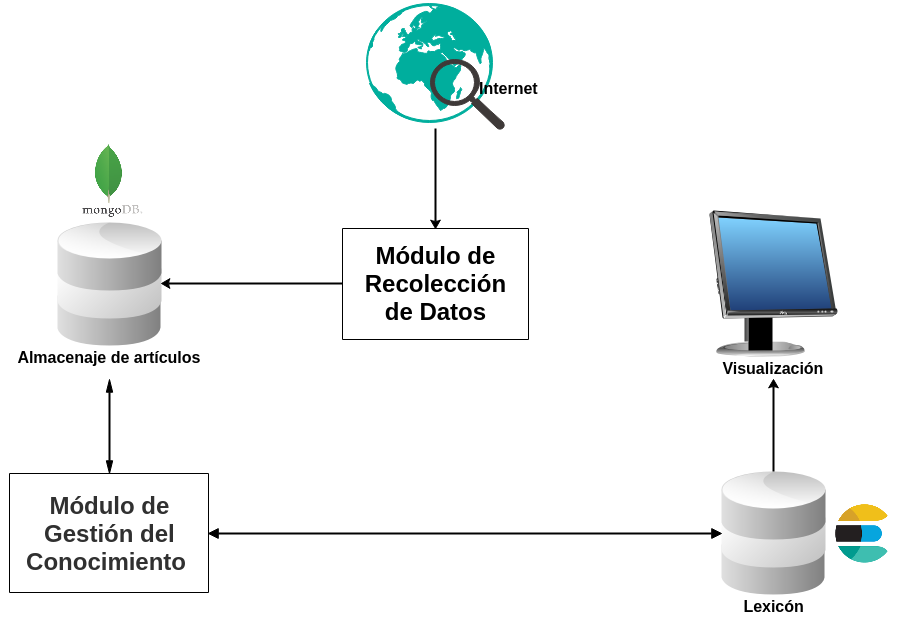
\includegraphics[width=10.2cm, keepaspectratio]{arquitectura.png}
\end{figure}
\end{frame}

\subsection{Módulo de recolección y preparación de datos}
\begin{frame} \frametitle{Descarga y limpieza de datos} 
\begin{itemize}
\item Descarga, limpieza y parseo de artículos.
\item Cálculo de resúmenes automáticos.
\item Cálculo de reputaciones.
La reputación de un artículo viene dada por la siguiente fórmula:
\begin{equation}
	rep_{p} = \alpha * 	rep\_authors_{p}  + (1 - \alpha) * citations_{p} \,,
\end{equation}
\begin{equation}\label{eq:1}
	rep\_authors_{p} = \sum  \limits_{i=1}^n  rep_{i} / n \,.
\end{equation}
\begin{equation}
	rep_{i} = \omega_1 * inf\_citation\_count + \omega_2 * citation\_velocity + \omega_3 * seniority + \omega_4 * papers \,,
    \label{eq:author_reputation}
\end{equation}


\end{itemize}

\end{frame}

\begin{frame} \frametitle{Descarga y limpieza de datos} 
\begin{table}[]
\begin{center}

\begin{tabular}{|c|c|}
\hline
\textbf{Parámetro}       & \textbf{Saturación} \\ \hline
Número de artículos      & 196                 \\ \hline
citationVelocity         & 105                 \\ \hline
influentialCitationCount & 208                 \\ \hline
Seniority                & 34                  \\ \hline
Citas del artículo       & 10                  \\ \hline
\end{tabular}
\caption{Valores de saturación de parámetros de reputación}
\label{tab:saturacion}
\end{center}
\end{table}

\end{frame}


\subsection{Módulo de gestión del conocimiento}
\begin{frame} \frametitle{Módulo de gestión del conocimiento} 
\begin{itemize}
\item Obtención de matriz de términos por documentos.
\item Creación del lexicón:
\begin{equation}
	relevance(t) =\log(\frac{1}{N} \sum  \limits_{i=1}^N \alpha \cdot tfidf(t_i) + (1-\alpha)\cdot reputation_i),    \forall t \in D
    \label{eq:relevance}
\end{equation}
\begin{equation}
	relevance'(t) = \beta \cdot relevance(t) + (1 - \beta) \cdot occurence(t)
    \label{eq:relevance2}
\end{equation}

\item Visualización
\item Evaluación de nuevos artículos:
\begin{equation}
	relevance_d =  \frac{1}{N} \sum  \limits_{i=1}^N relevance'(t_i)
    \label{eq:relevance3}
\end{equation}

\end{itemize}



\end{frame}


\section{Experimentos}
\subsection{}

\section{Trabajos futuros}
\begin{frame} \frametitle{Trabajos futuros} 
\begin{itemize}
\item Optimización del cálculo de relevancias para poder considerar un mayor corpus.
\item Implementar, probar y comparar otras métricas de relevancia.
\item Emplear relaciones jeraŕquicas de ontologías médicas.
\item Extracción de entidades con Scipacy
\item Construir lexicones por cada año.
\item Crear una red de neuronas para predecir las relevancias de los términos que no se encuentren en el lexicón.
\end{itemize}
\end{frame}


\end{document}